
%(BEGIN_QUESTION)
% Copyright 2010, Tony R. Kuphaldt, released under the Creative Commons Attribution License (v 1.0)
% This means you may do almost anything with this work of mine, so long as you give me proper credit

Determine the value of the specified {\it integral} for this function:

$$\includegraphics[width=15.5cm]{i04377x01.eps}$$

$$\int_{8}^{-4} f(x) \> dx$$

\underbar{file i04377}
%(END_QUESTION)





%(BEGIN_ANSWER)

$-10.14$

\vskip 10pt

This is another example where the interval of integration specifies a negative direction (i.e. each differential $dx$ is a negative quantity).  This explains why the integral value is {\it negative} 10.14 rather than positive, even though the enclosed area above the zero line exceeds the enclosed area below the zero line.

%(END_ANSWER)





%(BEGIN_NOTES)


%INDEX% Mathematics, calculus: integral (approximating integral values between points on graph)

%(END_NOTES)


